\chapter{Distance Matching: Theory and Experiments}

\begin{goals}
\begin{itemize}
    \item Formalize the distance matching principle
    \item Connect it to optimization theory via condition number
    \item Verify empirically with diverse architectures and tasks
    \item Show that loss function induces the behavioral metric
\end{itemize}
\end{goals}

\section{The Core Principle}

\begin{keyinsight}
\textbf{Distance Matching Principle}: A parameterization $\gamma: \Theta \to \mathcal{F}$ is ``good'' if parameter distance is proportional to function distance:
\[
c_1 \cdot d_\Theta(\theta_1, \theta_2) \leq d_{\mathcal{F}}(\gamma(\theta_1), \gamma(\theta_2)) \leq c_2 \cdot d_\Theta(\theta_1, \theta_2)
\]
When $c_1 \approx c_2$, the mapping is approximately an isometry.
\end{keyinsight}

\section{Loss Function Induces Behavioral Metric}

A key insight: the loss function \emph{defines} the behavioral metric, not the other way around.

For MSE loss $L(\theta) = \|f_\theta(X) - Y\|_2^2$, the natural behavioral distance is:
\[
d_{\text{behavior}}(f, g) = \|f(X) - g(X)\|_2
\]

This is not an arbitrary choice---it is \emph{induced} by the loss function:

\begin{center}
\begin{tabular}{lll}
\textbf{Loss Function} & \textbf{Output Metric} & \textbf{Behavioral Distance} \\
\hline
MSE & $L_2$ & $\|f(X) - g(X)\|_2$ \\
MAE & $L_1$ & $\|f(X) - g(X)\|_1$ \\
Cross-entropy & KL divergence & $D_{KL}(f \| g)$ \\
Wasserstein & Wasserstein & $W(f, g)$ \\
\end{tabular}
\end{center}

\begin{keyinsight}
The loss function simultaneously defines:
\begin{enumerate}
    \item What we optimize (minimize loss)
    \item The behavioral metric (distance on function space)
\end{enumerate}
These are two sides of the same coin.
\end{keyinsight}

\section{Connection to Optimization: The Jacobian}

Let $J = \frac{\partial f_\theta(X)}{\partial \theta}$ be the Jacobian of the parameter-to-output mapping.

\subsection{Condition Number}

The \textbf{condition number} $\kappa(J) = \sigma_{\max}(J) / \sigma_{\min}(J)$ measures how well distances are preserved:
\begin{itemize}
    \item $\kappa(J) = 1$: perfect isometry
    \item $\kappa(J)$ large: some directions stretched, others compressed
    \item $\kappa(J) = \infty$: null space exists (redundant parameters)
\end{itemize}

\subsection{Why $\kappa(J)$ Determines Learnability}

For MSE loss, the Hessian (Gauss-Newton approximation) is $H \approx J^\top J$.

\begin{theorem}
Gradient descent converges at rate $O\left(\left(1 - \frac{1}{\kappa(H)}\right)^t\right)$, where $\kappa(H) = \kappa(J)^2$.
\end{theorem}

Therefore:
\[
\kappa(J) \text{ small} \implies \kappa(H) \text{ small} \implies \text{fast convergence}
\]

\begin{keyinsight}
$\kappa(J)$ is the \textbf{precise measure of learnability}:
\begin{itemize}
    \item $\kappa(J)$ small $\to$ gradient descent converges quickly
    \item $\kappa(J)$ large $\to$ convergence is slow or unstable
\end{itemize}
\end{keyinsight}

\section{Experimental Verification}

We conducted extensive experiments to verify the theory.

\subsection{Experiment 1: Same Function Space, Different Parameterizations}

All models below express the \emph{same} function space (linear functions), but with different parameterizations:

\begin{center}
\begin{tabular}{lccc}
\textbf{Parameterization} & $\kappa(J)$ & \textbf{Final Loss} & \textbf{CV} \\
\hline
Direct: $f(x) = x \cdot \theta$ & 1.5 & 0.0000 & 0.00 \\
Redundant: $f(x) = x \cdot (a - b)$ & $\infty$ & 0.0000 & 0.00 \\
2-layer: $f(x) = x \cdot W_1 \cdot W_2$ & $\infty$ & 0.1390 & 1.29 \\
MLP (overkill) & $\infty$ & 2.5360 & 0.38 \\
\end{tabular}
\end{center}

Key observation: same function space, but parameterization determines $\kappa(J)$ and learning stability.

\subsection{Experiment 2: Depth Destroys Distance Matching}

Even for \emph{linear} networks (no nonlinearity), depth introduces implicit redundancy:

\begin{center}
\begin{tabular}{lcc}
\textbf{Model} & $\kappa(J)$ & \textbf{Rating} \\
\hline
1-layer linear & 1.9 & Excellent \\
2-layer linear ($W_2 W_1 x$) & $\infty$ & Poor \\
3-layer linear & $\infty$ & Poor \\
\end{tabular}
\end{center}

Why? Because $W_2 \cdot W_1 = W_2' \cdot W_1'$ has infinitely many solutions.

\subsection{Experiment 3: Classic Task-Architecture Matches}

When architecture matches task structure, $\kappa(J)$ is small:

\begin{center}
\begin{tabular}{llccc}
\textbf{Task} & \textbf{Architecture} & $\kappa(J)$ & \textbf{Loss} & \textbf{CV} \\
\hline
Permutation invariant $\sum x_i$ & DeepSets & \textbf{1.0} & 0.0000 & 0.87 \\
Multiplication $x_1 \cdot x_2$ & Mult gate & \textbf{1.0} & 0.0000 & \textbf{0.00} \\
Counting $\#(x > 0)$ & Counter & \textbf{1.0} & 0.1010 & 0.05 \\
Sparse $x_0 + x_1$ & Sparse (2 params) & \textbf{1.2} & 0.0000 & 0.78 \\
\hline
Linear & MLP & $\infty$ & 2.54 & -- \\
Permutation invariant & MLP & 336 & 2.02 & -- \\
Sparse & MLP & 60 & 1.08 & -- \\
\end{tabular}
\end{center}

The multiplication gate achieves \textbf{perfect} distance matching: $\kappa = 1$, loss $= 0$, CV $= 0$.

\subsection{Experiment 4: $\kappa(J)$ Determines Distribution of Outcomes}

We ran 30 random seeds for each architecture:

\begin{center}
\begin{tabular}{lcccc}
\textbf{Architecture} & $\kappa(J)$ & \textbf{Mean Loss} & \textbf{Std Loss} & \textbf{CV} \\
\hline
Linear direct & 1.5 & 0.008 & 0.000 & \textbf{0.00} \\
Linear (a-b) & $\infty$ & 0.008 & 0.000 & \textbf{0.00} \\
MLP 2-layer & $\infty$ & 0.59 & 0.57 & \textbf{0.96} \\
ResNet 2-layer & 15667 & 0.11 & 0.03 & 0.26 \\
\end{tabular}
\end{center}

\begin{keyinsight}
$\kappa(J)$ determines not a single convergence speed, but the \textbf{distribution} of outcomes:
\begin{itemize}
    \item $\kappa(J)$ small $\to$ narrow distribution (all seeds converge well)
    \item $\kappa(J)$ large $\to$ wide distribution (depends on luck/initialization)
\end{itemize}
This explains why ``good architectures'' are robust to initialization.
\end{keyinsight}

\section{Two Failure Modes}

An architecture can fail in two ways:

\begin{enumerate}
    \item \textbf{Lack of expressiveness}: Cannot represent the target function.
    \begin{itemize}
        \item Example: Linear model for multiplication
        \item Symptom: $\kappa(J)$ small but loss high
    \end{itemize}

    \item \textbf{Redundancy}: Can represent but has unnecessary parameters.
    \begin{itemize}
        \item Example: MLP for linear function
        \item Symptom: $\kappa(J)$ large, training unstable
    \end{itemize}
\end{enumerate}

The ideal architecture has:
\[
\text{Sufficient expressiveness} + \text{No redundancy} = \kappa(J) \text{ minimized}
\]

\section{Connection to Category Theory}

The framework connects to enriched category theory:

\begin{enumerate}
    \item \textbf{Loss function} defines the enrichment (metric on output space)
    \item This induces a \textbf{Lawvere metric} on the function space
    \item Distance matching asks: is $\gamma: \Theta \to \mathcal{F}$ a bi-Lipschitz map?
    \item $\kappa(J)$ is the Lipschitz constant ratio
\end{enumerate}

\begin{center}
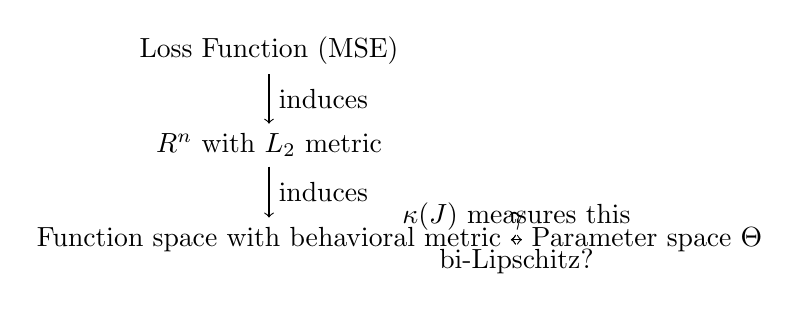
\begin{tikzpicture}[scale=1.2]
\node (loss) at (0, 2) {Loss Function (MSE)};
\node (output) at (0, 1) {$\mathbb{R}^n$ with $L_2$ metric};
\node (func) at (0, 0) {Function space with behavioral metric};
\node (param) at (4, 0) {Parameter space $\Theta$};

\draw[->] (loss) -- node[right] {induces} (output);
\draw[->] (output) -- node[right] {induces} (func);
\draw[->] (param) -- node[above] {$\gamma$} (func);
\draw[<->] (param) -- node[below] {bi-Lipschitz?} node[above] {$\kappa(J)$ measures this} (func);
\end{tikzpicture}
\end{center}

\section{Summary}

\begin{enumerate}
    \item \textbf{Behavioral metric} is induced by the loss function (not arbitrary)
    \item \textbf{Distance matching} = parameter distance $\approx$ behavioral distance
    \item \textbf{$\kappa(J)$} is the precise measure of distance matching quality
    \item \textbf{$\kappa(J)$ small} $\Leftrightarrow$ fast, stable learning
    \item \textbf{$\kappa(J)$ large} $\Leftrightarrow$ slow, unstable, seed-dependent
    \item \textbf{Good architecture} = matches task structure = minimizes $\kappa(J)$
\end{enumerate}

This provides a principled answer to ``why does architecture matter'': the right architecture achieves distance matching, making optimization efficient.

\section{Related Work}

The ideas in this chapter have deep connections to existing literature.

\subsection{Dynamical Isometry (Saxe et al., 2013)}

The concept of $\kappa(J) \approx 1$ was introduced as \textbf{dynamical isometry}:
\begin{quote}
``When the singular values of the input-output Jacobian are all clustered around one, the network achieves dynamical isometry and trains efficiently despite being very deep.''
\end{quote}

Key results:
\begin{itemize}
    \item Orthogonal initialization achieves dynamical isometry
    \item Deep linear networks can have depth-independent learning times with proper initialization
    \item This explains why certain initializations work better than others
\end{itemize}

\subsection{Neural Tangent Kernel (NTK) Theory}

The NTK literature explicitly connects eigenvalues to trainability:
\begin{itemize}
    \item $\lambda_{\min}(\text{NTK})$ determines the slowest convergence direction
    \item The condition number $\kappa = \lambda_{\max}/\lambda_{\min}$ is used as a \textbf{trainability measure}
    \item Convergence rate is $O(e^{-\lambda_{\min} t})$ along the slowest eigenvector
\end{itemize}

\subsection{Natural Gradient (Amari, 1998)}

Amari's natural gradient addresses distance mismatch by correcting gradients:
\[
\tilde{\nabla} L = F^{-1} \nabla L
\]
where $F$ is the Fisher information matrix. This makes gradient descent behave \emph{as if} distances matched.

Our perspective: instead of correcting gradients, choose a parameterization where ordinary gradients already work well.

\subsection{Coalgebraic Behavioral Metrics}

The categorical framework for behavioral metrics is well-developed:
\begin{itemize}
    \item Given functor $H$, the Kantorovich/Wasserstein lifting defines a behavioral metric
    \item $d(s, t) = 0$ iff $s$ and $t$ are bisimilar
    \item This provides a principled way to define ``behavioral distance''
\end{itemize}

\subsection{Our Contribution}

What we add to the existing picture:
\begin{enumerate}
    \item \textbf{Loss function as primitive}: The loss function \emph{induces} the behavioral metric (not a separate choice)
    \item \textbf{Distribution perspective}: $\kappa(J)$ determines the \emph{distribution} of outcomes over random seeds, not just expected convergence
    \item \textbf{Task-architecture matching}: Systematic experiments showing that matching architecture to task structure minimizes $\kappa(J)$
    \item \textbf{Categorical connection}: Framing in terms of Lawvere metric spaces and bi-Lipschitz maps
\end{enumerate}

\section{Open Questions}

\begin{enumerate}
    \item Can we \textbf{compute} $\kappa(J)$ efficiently for large networks?
    \item Given a task, can we \textbf{derive} the optimal architecture that minimizes $\kappa(J)$?
    \item How does $\kappa(J)$ relate to \textbf{generalization}? (We only addressed optimization)
    \item For non-MSE losses, what is the correct behavioral metric?
    \item Can the coalgebraic behavioral metric framework give us new architectures?
\end{enumerate}
